%%%% ijcai18.tex



% These are the instructions for authors for IJCAI-18.
% They are the same as the ones for IJCAI-11 with superficical wording
%   changes only.
\documentclass{article}

% if you need to pass options to natbib, use, e.g.:
% \PassOptionsToPackage{numbers, compress}{natbib}
% before loading nips_2018

% ready for submission
\usepackage{nips_2018}

% Use the postscript times font!
\usepackage{times}
\usepackage{xcolor}
\usepackage{soul}
\usepackage[utf8]{inputenc}
\usepackage[small]{caption}

\usepackage{array}
\usepackage{amsmath}
\usepackage{amsthm}
\usepackage{amssymb}
\usepackage{graphicx}
\usepackage{subfigure}
\usepackage{xspace}
\usepackage{paralist}
\usepackage{multirow}
\usepackage{caption,latexsym}
\usepackage[ruled,vlined,oldcommands]{algorithm2e}
\usepackage{wrapfig}
\newcounter{theorem}
\newtheorem{corollary}{Corollary}
\newtheorem{definition}{Definition}
\newtheorem{example}{Example}
\newtheorem{lemma}{Lemma}
\newtheorem{proposition}{Proposition}
\newtheorem{thrm}{Theorem}

% the following package is optional:
%\usepackage{latexsym} 

% Following comment is from ijcai97-submit.tex:
% The preparation of these files was supported by Schlumberger Palo Alto
% Research, AT\&T Bell Laboratories, and Morgan Kaufmann Publishers.
% Shirley Jowell, of Morgan Kaufmann Publishers, and Peter F.
% Patel-Schneider, of AT\&T Bell Laboratories collaborated on their
% preparation.

% These instructions can be modified and used in other conferences as long
% as credit to the authors and supporting agencies is retained, this notice
% is not changed, and further modification or reuse is not restricted.
% Neither Shirley Jowell nor Peter F. Patel-Schneider can be listed as
% contacts for providing assistance without their prior permission.

% To use for other conferences, change references to files and the
% conference appropriate and use other authors, contacts, publishers, and
% organizations.
% Also change the deadline and address for returning papers and the length and
% page charge instructions.
% Put where the files are available in the appropriate places.
\newcommand{\eat}[1]{}

\title{Approximate Lifted Inference in MLNs using Neural Embeddings}

% Single author syntax


% Multiple author syntax (remove the single-author syntax above and the \iffalse ... \fi here)
\iffalse
\author{
First Author$^1$, 
Second Author$^2$, 
Third Author$^3$, 
\\ 
$^1$ First Affiliation \\
$^2$ Second Affiliation\\
$^3$ Third Affiliation  \\
%
first@email.address,
second@email.address,
third@email.address
}
% If your authors do not fit in the default space, you can increase it 
% by uncommenting the following (adjust the "2.5in" size to make it fit
% properly)
% \setlength\titlebox{2.5in}
\fi

\begin{document}

\maketitle
\begin{abstract}
Lifted inference has become the predominant approach to scaling up inference in Markov Logic Networks (MLNs). The main challenge with lifted inference methods is to find symmetries in the MLN. Though there has been a considerable amount of work over the last several years in computing symmetries for MLNs, exploiting approximate symmetries to its fullest possible extent is a challenging task. In this paper, we present a novel approach for symmetry detection based on a neural embedding for objects in the MLN, which we call Obj2vec. Specifically, Obj2vec embeds objects in a low-dimensional space, where symmetric objects are placed close together in this space. Our approach is particularly useful, since it does not require difficult-to-compute features for detecting symmetries, and more importantly it takes advantage of joint dependencies across multiple domains to detect more complex symmetries than is possible if we treat domains independently. Our experiments on several real-world benchmarks validate our hypothesis, and show that Obj2vec-based lifted inference is accurate, scalable and effective in detecting symmetries.
\end{abstract}
\section{Introduction}

Markov Logic Networks (MLNs)~\cite{domingos&lowd09} are well-known statistical relational models with intuitive semantics and powerful expressiveness. Specifically, MLNs represent both relational concepts as well as uncertainty using weighted first-order logic formulas. An MLN is a template for Markov networks, i.e., we can instantiate an MLN with objects from a real-world domain and generate Markov networks which represent probability distribution over relational worlds of the MLN. A key challenge with MLNs, as is now well-known, is to develop scalable inference methods for them.  In this regard, the idea of {\em lifted} inference has been a major advancement, where the idea is to utilize symmetries that exist in the MLN due to its template structure, in order to improve scalability of inference.

However, identifying symmetries in the MLN efficiently and effectively is non-trivial. Specifically, the Markov network representing the MLN distribution is usually very large, and it is often intractable to try to process the MLN directly using its underlying Markov network representation. Therefore, several previously developed lifted inference methods try to process the MLN without creating its {\em ground} Markov network. For instance, popular exact lifted inference methods such as FOVE~\cite{braz07}, PTP~\cite{gogate&domingos11b} and WKBMC~\cite{broeck&al11} develop {\em lifting} rules which identify symmetries in the MLN directly from the first-order structure of its formulas. Similarly, several lifted approaches have been proposed for approximate inference by utilizing symmetries within MCMC\cite{niepert12,venugopal&gogate12}, belief propagation~\cite{singla&domingos08,ahmadi&al13}, etc.

Unfortunately, it turns out that exact symmetries required for lifted inference are usually absent in real-world MLNs. Therefore, a relatively new direction has been to use approximate symmetries to perform lifted inference in a scalable manner on real-world MLNs. Broeck and Darwiche~\cite{broeck&darwiche13} proposed a boolean factorization approach to approximate binary evidence with evidence that has more symmetries, which makes lifting easier. Venugopal and Gogate~\cite{venugopal&gogate14} proposed a pre-processing method that clusters each domain using algorithms such as K-Means, and then replaces a cluster by its cluster-center. However, there are some key issues with these approximate lifting methods. First, clustering methods such as K-Means requires feature-engineering. For example, Venugopal and Gogate use features based on counts of formulas satisfied by the evidence. Such features need to accurately encode symmetry in the MLN. Second, joint dependencies between across domains in the MLN are not fully considered while learning the approximate symmetries. For example, consider an MLN that analyzes restaurant reviews. The likelihood of symmetry between two distinct reviews increases if the reviews are written for restaurants that have symmetry. At the same time,  restaurants that are somewhat similar may elicit reviews that have a higher likelihood of symmetries. Our main contribution in this paper is to significantly advance the state-of-the-art in detecting approximate symmetries in MLNs by using neural embeddings. Two key advantages of our approach include, it does not use any hand-coded features, and it takes advantage of joint dependencies across domains to detect symmetries more effectively.

Our approach is based on the premise that objects that have similar contexts in the MLN formulas exhibit symmetries. For example, consider once again, the domain of reviews written for restaurants. If, in the ground formulas of the MLN, whenever a ground formula containing review $R_1$ is true, and a ground formula containing review $R_2$ is true, if the other objects in the ground formulas such as restaurants, users, etc. (which forms the context for $R_1$ and $R_2$) are symmetric, then it is likely that $R_1$ and $R_2$ are also symmetric. To detect such symmetries, we develop a novel model similar to the popular skip-gram models (such as Word2vec) which we call Obj2vec model. Obj2vec encodes the context in which objects appear in a ground formula of the MLN that is satisfied by the observed evidence, as ``sentences'', and then generates a low-dimensional embedding for these objects. Objects that have similar contexts will be close to each other in the embedded vector-space, and are therefore considered as approximately symmetric to each other. We reduce the total number of objects in the domains of the MLN by removing a subset of objects whose vectors are close to the vectors of objects that we retain in the MLN. As is the case with previous approaches~\cite{broeck&darwiche13,venugopal&gogate14}, since our approach is a pre-processing method on the MLN, it can be applied to scale-up any existing inference algorithm.


%Thus, if two objects (corresponding to possibly different domains) share a common formula, since these objects appear together in a similar context in the MLN, our encoding places them close to each other in the document. This has the effect that distinct objects of a domain that appear in a common context are likely to be symmetrical to each other since they interact with similar objects. We then use Word2vec to vectorize each object, where distinct objects that consistently appear in similar contexts are likely to be close to each other in the vector space. We reduce the total number of objects in the MLN by removing a subset of objects whose vectors are close to the vectors of objects retained in the MLN. Since our approach is a pre-processing method, it can be applied to scale-up any inference algorithm.

We perform experiments on three real-world datasets taken from Alchemy~\cite{kok&al06}, namely, Webkb for collective classification, Cora for entity resolution, and protein interaction. Further, to illustrate the value of our approach in detecting symmetries, we use a dataset containing Yelp reviews from restaurants. We show that our approach significantly outperforms existing approaches and is effective in detecting symmetries from context.







\section{Background}
\subsection{Markov Logic Networks} Markov logic networks (MLNs) are template models that define uncertain, relational knowledge as first-order formulas with weights. Weights encode uncertainty in a formula. $\infty$ weight formulas are hard constraints which should always be true. Similarly formulas with $-\infty$ weights are always false. Thus, MLNs offer a flexible framework to mix hard and soft formulas. In MLNs, we assume that each argument of each predicate in the MLN is typed and can only be assigned to a finite set of constants. By extension, each logical variable in each formula is also typed. Thus, each variable corresponds to a specific domain of objects. A ground atom is an atom where each of its variables have bee substituted by constants from their respective domains. A ground formula is a formula containing only ground atoms.

Given a set of constants that represent the domains of variables in the MLN, an MLN represents a factored probability distribution over the possible worlds, in the form of a Markov network. A world in an MLN is an assignment of 0/1 to all ground atoms of the MLN. Specifically, the distribution is given by,
 \begin{align} \Pr(\omega) &
= \frac{1}{Z} \exp \left ( \sum_{i} w_i N_{i}(\omega) \right ) \label{eq:mln_prob_dist}
\end{align} where $w_i$ is the weight of formula $f_i$, $N_{i}({\omega})$ is the number of groundings of formula $f_i$ that evaluate to True given a world
$\omega$, and $Z$ is the normalization constant.

The two common inference problems over MLNs are (1) given observed evidence, compute the marginal probability distribution of a ground atom in the ground Markov network (2) given observed evidence, compute the most probable assignment to all non-evidence atoms. Both queries are computationally hard, and therefore require approximate inference methods.
\eat{
Important inference queries in MLNs are computing the partition function, finding the
marginal probability of an atom given evidence (an assignment to a subset of variables) and finding
the most probable assignment to all atoms given evidence (MAP inference). Here, we focus on the marginal inference problem.
}
\eat{
As a simple example of an MLN, suppose we want to encode the fact that smokers and asthmatics are not friends. We would design an MLN with a formula such as $\texttt{Smokes}(x)$ $\wedge$ $\texttt{Friends}(x,y)$ $\Rightarrow$ $\neg Asthma(y)$. Given constants corresponding to the variables, $x$ and $y$, the MLN represents a joint distribution over all ground atoms of $\texttt{Smokes}$, $\texttt{Friends}$, and $\texttt{Asthma}$. The two key tasks in MLNs are {\em weight learning}, which is the task of learning 
the weights attached to the formulas from a relational database, and {\em inference} (prediction),
which is the task of answering queries posed over the learned model given observations (evidence database).
The two main inference problems over MLNs are (1) posterior or marginal estimation which involves finding the marginal probability distribution of a random variable (ground atom) in the ground Markov network given an evidence database. For example computing the probability that $\texttt{Smokes}(Ana)$ is true given $\texttt{Smokes}(Bob)$ is true and $\texttt{Friends}(Ana, Bob)$ is true. (2) Maximum-a-posteriori (MAP) estimation which involves finding an assignment of values to all non-evidence variables such that the assignment has the maximum probability. For example, given that $\texttt{Smokes}(Ana)$, $\texttt{Smokes}(Bob)$ and $\texttt{Friends}(Ana, Bob)$ is true, what is the assignment to all other ground atoms in the MLN such that their joint probability is maximum.

Both marginal inference and MAP inference are \#P-hard and NP-hard in general respectively. Several interesting tasks such as structured prediction and joint inference are special cases of these inference tasks. 
Weights attached to first-order formulas can be learned either {\em generatively}, in which the goal is to find weights that maximize the log-likelihood of the data, or {\em discriminatively}, in which the goal is to maximize the conditional log-likelihood of the data given evidence. In principle, both tasks can be solved using a standard gradient ascent procedure with appropriate regularization constraints. However, it turns out that computing the gradient is computationally intractable, since the problem of computing the gradient can be reduced to the posterior marginal estimation task. Therefore, practitioners often use alternate objective criteria such as contrastive divergence \cite{hinton02}, voted perceptron \cite{collins02}, and pseudo log-likelihood \cite{besag75} since the gradient of these functions is easier to compute.
}

\subsection{Skip-Gram Models}

Skip-gram models are used to learn an embedding over words based on the context in which they appear in the training data (i.e., neighboring words). Word2vec~\cite{mikolov&al13} is a popular model of this type, where we train a neural network based on pairs of words seen in the training data. Specifically, we use a sliding window of a fixed size, and generate all pairs of words within that sliding window. For each pair of words, we present one word of the pair as input, and the other word as a target. That is, we learn to predict a word based on its context or neighboring words. The hidden layer typically has a much smaller number of dimensions as compared to the input/output layers. Thus, the hidden-layer learns a low-dimensional embedding that is capable of mapping words to their contexts. Typically the hidden-layer output is used as features for other text processing tasks, as opposed to using hand-crafted features.
\subsection{Related Work}

Lifted inference methods exploiting exact symmetries have been explored in several earlier works in the context of exact inference (\cite{poole03,braz07,gogate&domingos11b,broeck&al11}) as well as approximate inference (\cite{singla&domingos08,niepert12,venugopal&gogate12}). Further, the idea of using approximate symmetries for inference has been used to develop general pre-processing methods such as using boolean factorization to generate a symmetric approximation of evidence~\cite{broeck&darwiche13}, and clustering domain objects to reduce the MLN size~\cite{venugopal&gogate14}. More recently, approximate symmetries have been used in specific inference algorithms, such as MAP inference~\cite{sarkhel&al15}, sampling-based inference~\cite{broeck&niepert15}, and linear programming~\cite{kersting&al17}. Kopp et al.~\cite{kopp&al15} used symmetry breaking techniques commonly used in the SAT community and applied it to lifted inference. More recently, Anand et al. ~\cite{anand&al16,anand&al17}proposed the use of non-count symmetries, and contextual symmetries in graphical models. Specifically, they used graph-based tools to detect automorphism groups, and infer symmetries from such groups. There has also been several previous works that have focussed on learning embeddings for relational data~\cite{bordes&al11}. However, to the best of our knowledge, ours is the first work to consider lifted inference using neural embeddings.
\section{Lifted Inference using Embeddings}

We generate a low-dimensional neural embedding for the MLN objects using a model we call Obj2Vec, where approximately symmetric objects lie close to each other in the embedding. 
%To achieve this, we encode objects in the MLN that share a ground formula as sentences, and run Word2vec to this encoding to learn the symmetry between objects, using which we can reduce the number of objects in the MLN.
%. Specifically, the general idea behind our approach is that symmetric objects share similar contexts in the MLN formulas. Therefore, learning a low-dimensional embedding  for the objects based on their context will
%Specifically,  symmetric objects in the MLN are likely to be close to each other in the embedded vector-space. To achieve this, we encode objects that share a ground formula in the MLN as sentences such that symmetrical objects yield similar sentences in our model. We next run Word2vec on the encoded objects to generate their embedding in a lower dimension. 
To formalize our approach, we assume that our MLN has $n$ domains $\Delta_1$, $\Delta_2$ $\ldots$ $\Delta_n$.  Let $\mathcal{D}$ be the evidence database presented to the MLN,  $f_1$ $\ldots$ $f_k$ be the MLN formulas, and ${\tt R}_1$ $\ldots$ ${\tt R}_p$ be the predicates. Our task is to embed the set of domains $\Delta_1$, $\Delta_2$ $\ldots$ $\Delta_n$ into a lower-dimensional space, and use similarity of the objects in the embedded space to reduce the size of the domains, and create a new domain-set $\hat{\Delta}_1$, $\hat{\Delta}_2$ $\ldots$ $\hat{\Delta}_n$, where $|\hat{\Delta}_i|$ $\leq$ $|{\Delta}_i|$.
 
 \subsection{Obj2Vec}
\begin{figure} 
\centering
 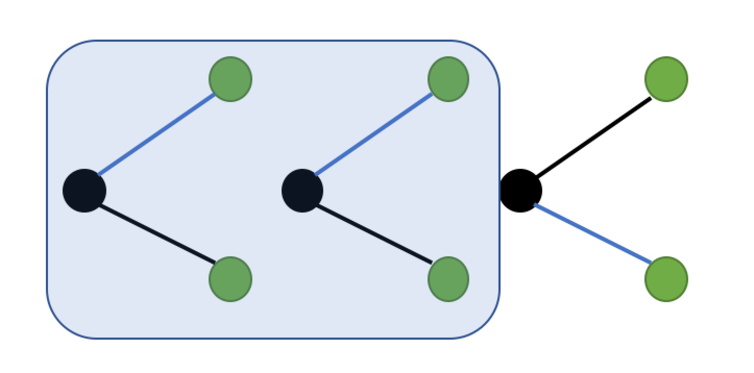
\includegraphics[scale=0.55]{ex1.pdf}
 \caption{\label{fig:ex1}Markov network for ${\tt R}(x)$ $\wedge$ ${\tt S}(x,y)$. The green nodes correspond to ${\tt S}$ and black nodes to ${\tt R}$. The blue line indicates that the grounding corresponding to that potential is satisfied by the evidence given by ${\tt R}(X_1)$, ${\tt R}(X_2)$, ${\tt R}(X_3)$, ${\tt S}(X_1,Y_1)$, ${\tt S}(X_2,Y_1)$, ${\tt S}(X_3,Y_2)$. The groundings corresponding to $X_1$ and $X_2$ are symmetric.}
 \end{figure}
 
 
Consider a simple formula ${\tt R}(x)$ $\wedge$ ${\tt S}(x,y)$. Let $\Delta_x$ $=$ $\{X_1,X_2,X_3\}$ and $\Delta_y$ $=$ $\{Y_1,Y_2\}$. Let the evidence database be ${\tt R}(X_1)$, ${\tt R}(X_2)$, ${\tt R}(X_3)$, ${\tt S}(X_1,Y_1)$, ${\tt S}(X_2,Y_1)$, ${\tt S}(X_3,Y_2)$. The objects $X_1$ and $X_2$ are symmetrical since they can be exchanged in the groundings in which they appear without changing the MLN as shown in Fig.~\ref{fig:ex1}. Specifically, they appear  along with similar objects (in this case $Y_1$) in ground formulas of the MLN. Using this, we can define the context as follows.

 \begin{definition}
 Let $\bar{f}$ be a ground formula satisfied by evidence $\mathcal{D}$. We define the context of any object in $\bar{f}$  as the set of other objects in $\bar{f}$ .
 \end{definition}

Our idea is to detect symmetries based on the above-defined context. For this, consider the following encoding for the MLN objects, where for every satisfied ground formula, we list the objects that appear in the context of each other. Therefore, for our previous example, the encoding is, $X_1Y_1;X_2Y_1;X_3Y_2$. Analogous to the input to skip-gram models, we can think of each ground formula as being encoded as a ``sentence'' in a document, where the sentences are shown to be separated by a ``;'. The pair $X_1Y_1$ encodes that $X_1$ has a context $Y_1$ in some grounding of the MLN formula. Notice that $X_2$ also has a context $Y_1$.

%Clearly, the objects $X_1$ and $X_2$ are symmetrical since they  



%Clearly, the ground formulas ${\tt R}(X_1)$ $\wedge$ ${\tt S}(X_1,Y_1)$ and ${\tt R}(X_2)$ $\wedge$ ${\tt S}(X_2,Y_1)$ are symmetrical due to the evidence presented. context in which these objects appear. Specifically, both $X_1$ and $X_2$ appear along with $Y_1$ 


%Consider the following encoding of the MLN, $X_1Y_1;X_2Y_1;X_3Y_2$, where sentences are shown to be separated by a ``;''. The pair $X_1Y_1$ encodes that $X_1$ has a dependency with $Y_1$ in some grounding of the MLN formula. Notice that $X_2$ also has a dependency with $Y_1$. Thus, $X_1$ and $X_2$ are symmetrical to each other. 

Now let us consider a neural network architecture that will work on our input encoding. Specifically, the network architecture we use is the same as is used in skip-gram models such as Word2Vec. For Word2vec, the context is defined by a small fixed-size window of words in a document, while for Obj2vec, the context is the objects in a ground formula that is satisfied by the evidence. Therefore, just as in skip-gram models, from each of our encoded sentences $X_1Y_1$, $X_2Y_1$ and $X_3Y_2$, we generate input/output pairs, where we predict an object given another object from its context. That is, given $X_1$ or $X_2$ at the input layer, we predict $Y_1$ at the output layer, and given $X_3$ as input we predict $Y_2$ as the output layer. This means that the hidden layer in the model will derive features such that $X_1$ and $X_2$ will make common predictions at the output layer. Therefore, the hidden layer representation for both $X_1$ and $X_2$ should be similar indicating symmetry of $X_1$ and $X_2$. As the context surrounding both $X_1$ and $X_2$ becomes more and more similar, the embedding for $X_1$ and $X_2$ grows closer to each other.  At the same time, since $X_3$ has a different context, it needs to predict $Y_2$ at the output layer, and therefore, the hidden layer encoding for $X_3$ will be different from that of $X_1$ and $X_2$. 
%Now, say $X_3$ relates with common objects as $X_1$ and $X_2$ on other groundings on the MLN, the hidden layer embedding for $X_3$ will grow closer to that of $X_1$ and $X_2$ indicating symmetry between the objects.

\begin{figure} 
\centering
 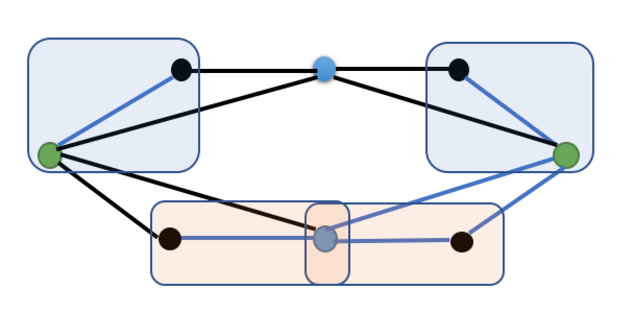
\includegraphics[scale=0.65]{ex2.pdf}
 \caption{\label{fig:ex2}Markov network for ${\tt R}(x)$ $\wedge$ ${\tt S}(x,y)$ $\wedge$ ${\tt T}(y)$. The green nodes correspond to ${\tt R}$, black nodes to ${\tt S}$ and blue nodes to ${\tt T}$. The blue line indicates that the partial grounding corresponding to that potential is satisfied by the evidence given by ${\tt R}(X_1)$, ${\tt S}(X_1,Y_1)$, ${\tt R}(X_2)$, ${\tt S}(X_2,Y_1)$, ${\tt S}(X_2,Y_2)$, ${\tt T}(Y_2)$. Symmetries are shown as shaded regions.}
 \end{figure}

To generalize the above, let $D$ be the ``document'' we generate from $\Delta_1$, $\Delta_2$ $\ldots$ $\Delta_n$  by encoding the object contexts as sentences. Let $\bar{f}_i^j$ be the $j$-th grounding of the $i$-th formula. We now have two cases, $\bar{f}_i^j$ is satisfied by the evidence $\mathcal{D}$, or $\bar{f}_i^j$  is unsatisfied by $\mathcal{D}$. If $\bar{f}_i^j$ is satisfied by $\mathcal{D}$, we encode the the ground objects in $\bar{f}_i^j$ as a sentence in  $D$, indicating the context of the objects in $\bar{f}_i^j$. If $\bar{f}_i^j$ is not satisfied by $\mathcal{D}$, then we do not encode it in $D$. This is because, the context is not supported by the observed evidence. 

\noindent{\bf Partial Symmetries}. One of the consequences of encoding context only based on formulas satisfied by $\mathcal{D}$ is that we lose symmetries of partially satisfied formulas. For example, consider the following MLN, ${\tt R}(x)$ $\wedge$ ${\tt S}(x,y)$ $\wedge$ ${\tt T}(y)$. Let our evidence be ${\tt R}(X_1)$, ${\tt S}(X_1,Y_1)$, ${\tt R}(X_2)$, ${\tt S}(X_2,Y_1)$, ${\tt S}(X_2,Y_2)$, ${\tt T}(Y_2)$. The Markov network corresponding to the MLN is shown in Fig.~\ref{fig:ex2}. As shown here, there are some partial symmetries, even though the ground formulas are not satisfied by the evidence. Using our aforementioned encoding, since only one ground formula is satisfied by $\mathcal{D}$, our encoding produced is $X_2Y_1$. Therefore we cannot detect the symmetries that exist between $X_1$ and $X_2$ w.r.t the predicates ${\tt R}$ and ${\tt S}$, and the symmetries between $Y_1$ and $Y_2$ w.r.t predicates ${\tt S}$ and ${\tt T}$. Therefore, we modify our approach slightly to make it more fine-grained by encoding the context for objects for every pair of predicates in the MLN. The idea is that, for a pair of predicates, if the evidence shows that objects share a context, then it is possible that there are some symmetries between those objects. That is, let ${\tt R}_i$ and ${\tt R}_j$ be a predicate pair. For every formula $f_i$ where both ${\tt R}_i$ and ${\tt R}_j$ occur, we eliminate all predicates from $f_i$ other than ${\tt R}_i$ and ${\tt R}_j$, along with their preceding logical connectives. For example, ${\tt R}_i(x,y)$ $\wedge$ ${\tt R}_k(y,z)$ $\Rightarrow$ ${\tt R}_j(z,x)$ reduces to ${\tt R}_i(x,y)$ $\Rightarrow$ ${\tt R}_j(z,x)$. For each grounding of the modified formula, if the evidence $\mathcal{D}$ satisfies the formula, we encode the objects in the grounding as a sentence in our document $D$. Note that dependencies on self-joined predicates can be naturally handled using this approach by pairing ${\tt R}_i$ with itself.

\begin{figure}
\subfigure[]{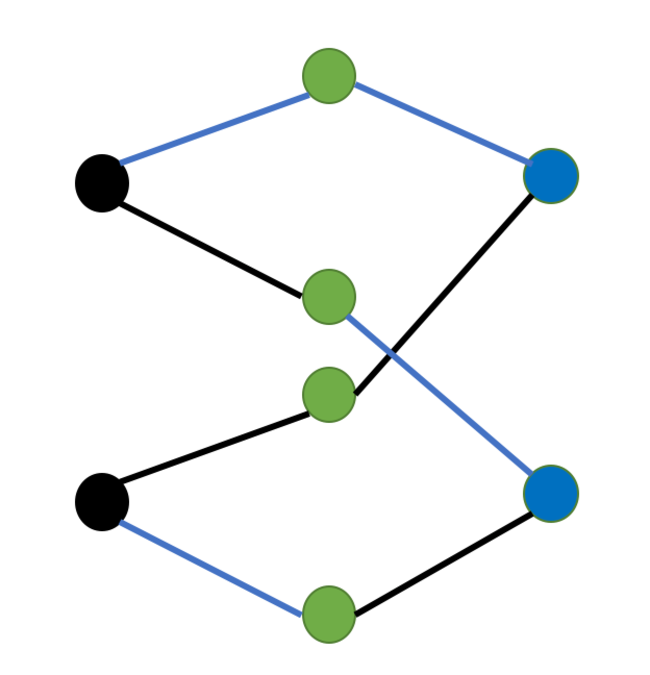
\includegraphics[scale=0.35]{ex3a.pdf}}
\subfigure[]{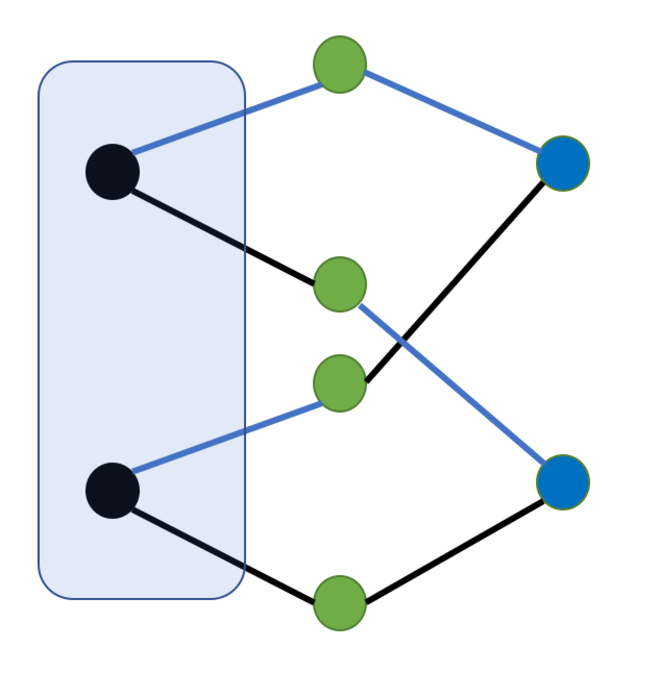
\includegraphics[scale=0.35]{ex3b.pdf}}
\caption{\label{fig:ex3}Markov network for ${\tt R}(x)$ $\wedge$ ${\tt S}(x,y)$; ${\tt S}(x,y)$ $\wedge$ ${\tt T}(y)$. The black nodes correspond to ${\tt R}$, green nodes to ${\tt S}$ and blue nodes to ${\tt T}$. The blue line indicates that the grounding corresponding to that potential is satisfied by the evidence. (a) shows the original Markov network. Due to the symmetries when we we consider the pair ${\tt S}$ and ${\tt T}$, we can interchange some of the links between ${\tt R}$ and ${\tt S}$, and detect symmetries on objects corresponding to $x$ as shown in (b).}
\end{figure}
\noindent{\bf Joint Symmetries}. One of the advantages of our approach is that symmetries on one object can affect symmetries on another object. For example, consider the formulas ${\tt R}(x)$ $\wedge$ ${\tt S}(x,y)$; ${\tt S}(x,y)$ $\wedge$ ${\tt T}(y)$. Suppose $Y_1$ and $Y_2$ appear in the same context w.r.t  ${\tt S}$ and ${\tt T}$ in several cases. The embedding for $Y_1$ and $Y_2$ will become similar in the hidden-layer of Obj2vec. Now suppose $X_1$ has a context $Y_1$, and $X_2$ has a context $Y_2$, then, due to the similarity of $Y_1$ and $Y_2$, even though $X_1$ and $X_2$ have differing contexts, the embedding for $X_1$ grows closer to $X_2$. This is illustrated in Fig.~\ref{fig:ex3}. Here (a) shows the Markov network for our example MLN given evidence ${\tt R}(X_1)$, ${\tt S}(X_1,Y_1)$, ${\tt R}(X_2)$, ${\tt S}(X_2,Y_2)$, ${\tt S}(X_1,Y_1)$, ${\tt S}(X_1,Y_2)$, ${\tt T}(Y_1)$, ${\tt T}(Y_2)$. Due to the symmetries on $Y_1$ and $Y_2$ (they both have same context $X_1$), we can exchange the color of the links between ${\tt R}(X_2)$, ${\tt S}(X_2,Y_1)$ and ${\tt R}(X_2)$, ${\tt S}(X_2,Y_2)$. This changes the the Markov network as shown in (b), and we can notice symmetries between $X_1$ and $X_2$. Thus, in general, we can propagate symmetries across domains, which would help us uncover more complex symmetries in the MLN that are hard to detect when independently clustering the domains.
%Specifically, let ${\tt P}$ and  ${\tt Q}$ be two predicates in our MLN. For every formula, we compute the dependencies between ${\tt P}$ and  ${\tt Q}$, and encode it in $D$. That is, for a formula $f_i$, we eliminate all predicates other than ${\tt P}$ and  ${\tt Q}$, along with the logical connective succeeding each of the eliminated predicates. For each grounding of the modified formula, if the evidence $\mathcal{D}$ satisfies the formula, we include the objects for which the formula is satisfied as a sentence in our document $D$. Note that dependencies on self-joined predicates can be naturally handled using this approach by pairing predicates with themselves.







%Let the evidence database be ${\tt R}(X_1,Y_1)$, ${\tt R}(X_1,Y_1)$, ${\tt R}(X_1,Y_1)$, ${\tt R}(X_1,Y_1)$, ${\tt S}(X_1,Y_1)$, ${\tt S}(X_2,Y_1)$, ${\tt S}(X_3,Y_2)$. 

%To do this, we encode the domain based on their relational dependencies with other domain objects in the MLN. 
%On the other hand, if our evidence database shows that, $X_1$ and $X_2$ 

%We now describe our approach to create a neural embedding of the MLN's domain. We would want objects that appear together with similar objects in MLN formulas to be close to each other in the embedded space. 

%For this, we encode groundings of MLN formulas as sentences in a document. 


%However, since considering all possible ground formulas is computationally expensive, we consider the interaction between subsets of predicates and compute our sentences from these subsets. We then use Word2vec to generate embeddings of objects, and reduce the objects based on the distance between object vectors in the embedded vector-space.

%\subsection{Encoding}

%Let ${\tt A}_1$ $\ldots$ ${\tt A}_m$ be the predicates in our MLN, let $\Delta_1$, $\Delta_2$ $\ldots$ $\Delta_n$ be the domains of the MLN computed from the evidence database $\mathcal{D}$. Let ${\bf X}$ be a possible subset of predicates of size $k$. For every formula $f$ in the MLN where ${\bf X}$ occurs, we compute the possible groundings for ${\bf X}$ from $f$, and encode them as sentences in our document. 
\eat{
\begin{example}
Let $w$ ${\tt R}(x)$ $\wedge$ ${\tt S}(x,y)$ be a single-formula MLN. We will 
\end{example}
}

%We consider all possible subset of predicates of size $k$, and encode the objects in $\Delta_1$, $\Delta_2$ $\ldots$ $\Delta_n$ as follows
\subsection{Reducing the Objects}

We reduce the number of objects in the MLN by reducing the number of symmetric objects. Let $\hat{\Delta}_i$  $\subseteq$ $\Delta_i$, and let $d(X_j,X_k)$ denote the distance between the vectors for $X_j$ and $X_k$ in the embedded vector-space, where $X_j$, $X_k$ $\in$ $\Delta_i$. We wish to find the subset $\hat{\Delta}_i$ such that the elements in $\hat{\Delta}_i$ are closest to elements in  $\hat{\Delta}'_i$ $=$ $\hat{\Delta}_i$ $\setminus$ $\hat{\Delta}_i$ in the embedded vector-space. Given a set $A$, let $\mathcal{N}(X,A)$ $=$ $\arg\min_{X'\in A}$ $d(X,X')$ . We define our objective for $\Delta_i$ to be,

\begin{equation}
\arg\min_{\hat{\Delta}_i\subseteq\Delta_i}\sum_{X\in\hat{\Delta}_i} d(X,\mathcal{N}(X,\hat{\Delta}'_i)
\end{equation}

with the constraint that $|\hat{\Delta}_i|$ $\leq$ $\alpha$. This is required to ensure that our chosen subset of objects is small enough to ensure feasibility of inference. The above problem is a special case of the weighted set-cover problem, and is therefore it is NP-hard to compute the optimal solution. Therefore, we approximate the solution using a greedy approach as follows. We start with an empty $\hat{\Delta}_i$. In each iteration, we sample an object from the pair of objects with closest distance and add it to $\hat{\Delta}_i$. Specifically, in each iteration $t$, we compute,


\begin{equation}
X^t = \arg\min_{X\in\hat{\Delta}'_i}d(X,\mathcal{N}(X,\hat{\Delta}'_i\setminus{X}))
\end{equation}

We now sample either $X^t$ or $\mathcal{N}(X^t,\hat{\Delta}'_i\setminus{X^t})$ with equal probability and add the sampled object, $\bar{X}^t$ to $\hat{\Delta}_i$. We now remove the non-sampled object along with its neighboring object from $\hat{\Delta}'_i$ in a recursive manner. That is, suppose the non-sampled object is $\bar{X}^t_0$, we remove $\bar{X}^t_0$, $\bar{X}^t_1$ $=$ $\mathcal{N}(\bar{X}^t_0,\hat{\Delta}'_i\setminus{\bar{X}^t_0})$, $\bar{X}^t_2$ $=$ $\mathcal{N}(\bar{X}^t_1,\hat{\Delta}'_i\setminus{\bar{X}^t_1})$, and so on. Thus, in each iteration, we remove a cluster of neighbors that are symmetric with the sampled object added to $\hat{\Delta}_i$. We denote the neighborhood of $\bar{X}^t$ by $\mathcal{H}(\bar{X}^t)$. All inference results obtained on $\bar{X}^t$ are assumed to hold for $\mathcal{H}(\bar{X}^t)$.

We stop adding elements to $\hat{\Delta}_i$ when $|\hat{\Delta}_i|$ $\geq$ $\alpha$. However, one problem with this greedy approach is that the solution may get struck in local optima. That is, we may add an element that is close to a few objects, and miss elements that may be symmetrical to many objects even though they may not be the closest pair during an iteration. To avoid local optima, we use a commonly used technique employed in methods such as MaxWalkSAT~\cite{kautz&al97b}. Specifically, we intersperse random walks in the solution-space along with the greedy iterations. That is, with probability $p$, we choose a pair $(X$, $\mathcal{N}(X,\hat{\Delta}'_i\setminus{X}))$, where $X$ $\in$ $\hat{\Delta}'_i$ uniformly at random, and sample an object with probability 0.5 from this pair. As before, we remove the non-sampled object and its neighbors recursively from $\hat{\Delta}'_i$. With probability $1-p$, we choose the pair from which we sample the object greedily.

Given the new domains $\hat{\Delta}_1$, $\ldots$ $\hat{\Delta}_k$, we change the evidence database $\mathcal{D}$, by removing all evidences that contain objects that are not in the new domains. We map the results obtained from inference using the new evidence database to inference results on the original MLN as follows. The inference results (marginal probability, MAP assignment, etc.) obtained after conditioning on the changed evidence, for an atom grounded with objects $X_1$ $\ldots$ $X_k$ is assumed to hold for all atoms in the original MLN grounded with objects $\mathcal{H}(X_1)$ $\times$ $\ldots$ $\times$ $\mathcal{H}(X_k)$.  Our complete approach is summarized in Algorithm 1.

\begin{algorithm}[!t]{
\label{alg:wvec}
\linesnumbered
\caption{Obj2Vec Lifting}
\KwIn{MLN structure $\mathcal{M}$, Evidence $\mathcal{D}$, Inference algorithm $\mathcal{I}$, embedding dimensions $m$, object bound $\alpha$}
\KwOut{Inference results $R$}
\tcp{Encoding}
\For{each predicate pair $({\tt R}_i,{\tt R}_j)$}
{
\For{each formula $f$ in $\mathcal{M}$} {
$f'$ $=$ Eliminate all atoms not corresponding to $({\tt R}_i,{\tt R}_j)$\\
Encode groundings of $f'$ satisfied by $\mathcal{D}$ as sentences in document $D$\\
}
}
\tcp{Embedding}
$H$ $=$ Learn a model from $D$ to create a $m$-dimension embedding\\
\tcp{Sampling Objects}
\For{each domain} {
$\Delta_i$ $=$ original domain\\
$\hat{\Delta}_i$ $=$ $\{\}$\\
\While{$|\hat{\Delta}_i|$ $\leq$ $\alpha$} {
$X^t$ $=$ With probability $p$, sample an object from $\Delta_i$ with the closest object-pair\\
$X^t$ $=$ With probability $1-p$, sample an object from $\Delta_i$ from an object-pair chosen uniformly at random\\
$\hat{\Delta}_i$ $=$ $X^t\cup \hat{\Delta}_i$
Remove $X^t$ and $\mathcal{H}(X^t)$ from $\Delta_i$\\
}
}
\tcp{Inference}
Convert $\mathcal{D}$ to $\mathcal{D}'$ using new domains $\hat{\Delta}_1$, $\ldots$ $\hat{\Delta}_n$\\
$R'$ $=$ Run $\mathcal{I}$ on $\mathcal{M}$ conditioning on $\mathcal{D}'$\\
$R$ $=$ Project $R$ on original atoms\\
return $R$\\
}
\end{algorithm}

%Therefore, we want to penalize those objects that have small neighborhoods. To do this, we form clusters of objects from  the 

%We now  remove the non-sampled object (either $X^t$ or $\mathcal{N}(X^t,\hat{\Delta}'_i\setminus{X^t})$) from $\hat{Delta}'_i$ . 
%for every object $X$ $\in$ $\hat{\Delta}_i$ $\setminus$ $\hat{\Delta}_i$, we compute $\mathcal{N}(X)$ and add $Y$ $\in$ $\hat{\Delta}_i$ $\setminus$ $\hat{\Delta}_i$

%Specifically, let $X_i,X_j\in\Delta_i$ and let $d(X_1,X_2)$ be the distance between the vector representations in the low-dimensional embedding for objects $X_1$ and $X_2$. 

%and let $\hat{\Delta}'_i$ be its complement, $\hat{\Delta}_i$ $\setminus$ $\hat{\Delta}_i$
\section{Experiments}

\subsection{Setup}
We conducted our experiments on three benchmarks, Webkb, ER and Protein, all of which are publicly available in Alchemy~\cite{kok&al06}. Further, we created a new dataset from Yelp reviews, and analyzed our approach with this dataset. We implemented Obj2Vec using the Gensim package~\cite{rehurek_lrec}.

\eat{
We first took 5$\%$ subsets of each benchmark which we consider as gold standard and refer as GS since original data cannot be run in the state-of-the-art MLN systems e.g. Tuffy~\cite{niu&al11} and Magician~\cite{magician16} which implements scalable versions of contrastive divergence (CD), voted perceptron (VP) and pseudo-log-likelihood maximisation (PLL), using approximate counting oracles~\cite{sarkhel&al16}. We generated compressed distribution of benchmarks using our neural embedding approach which we refer as NE, generated another compressed distribution using  another baseline method where we used Venugopal and Gogate's~\cite{venugopal&gogate14} approach (available in the Magician open-source code) and refer as VG. We generated another compressed distribution sampling evidence atoms randomly and refer to this as Random. So, each meta atom from compressed distributions represents multiple atoms of GS. We ran marginal inference on compressed datasets and GS in Magician which is available as open-source.
}

We compared our Obj2Vec-based lifting approach which we refer to as NE, with Venugopal and Gogate's~\cite{venugopal&gogate14} approach (VG) available in Magician~\cite{magician16}, where they compress the MLN using K-Means clustering, using features based on counts of formulas satisfied by the evidence. To make the comparison fair, we ensured that we reduced each domain to 10$\%$ of its original value in both NE as well as VG. For our Obj2vec architecture, we set the number of number of neurons in the hidden layer as $10\%$ of the total number of objects in the MLN. For a sanity check, we also added an alternative approach, which we refer to as Random, where we sample evidence atoms randomly to reduce the size of the MLN.

\eat{
We got marginal probabilities for query meta atoms while we ran marginal inference on compressed distributions and compared the resulting marginals with marginals of GS. We used a threshold value to determine atoms as true or false. Since each meta atom from compressed distribution represents multiple atoms of GS, we treated those atoms as true if that meta atom is true from marginal inference output and false if the meta atom is false and compared the marginal inference results of compressed distributions to GS and computed F-measure.
}

\eat{
We also experimented NE on review spam benchmark from Yelp where each review having a score is written by a user for a restaurant and each review contains some word which we represented by a simple MLN : ${\tt R}$ (review) $\wedge$ ${\tt S}$ (review,word) $\wedge$ ${\tt T}$ (review,user) $\wedge$ ${\tt U}$ (review,restaurant) $\wedge$ ${\tt V}$ (review,score). Then we applied our NE on this MLN with the purpose that symmetric reviews should have similar restaurants and users as NE considers joint dependency among domains.
}

\subsection{Results}

\eat{
We evaluated our approach on three key aspects, (i) Solution Assurance, (ii) Solution Quality, and, (iii) Scalability. To ensure that our idea is promising, we have created a synthetic benchmark where symmetry among domain objects can be easily detected and reported how  accurately our approach finds symmetries among objects as we increase number of formulas in MLN. For quality, we have reported F-measure of NE, VG and Random and finally, we have reported running time of each approach to ensure the scalability.
}
We evaluate our approach on the accuracy of inference, ability to detect symmetries, and scalability.
\subsubsection{Accuracy}
\eat{
We compared marginal inference result for NE, VG and Random with GS and computed F-measure for the benchmarks. Fig.~\ref{fig:quality} exhibits that our NE significantly outperforms both VG and Random for all of the benchmarks. We applied NE on review spam benchmark and picked 10 top symmetric reviews and tried to plot similarity scores of those reviews and also similarity scores of the respective users and restaurants. As we described earlier, symmetric reviews supposed to have symmetric users and restaurants which is reflected in Table~\ref{tab:score} and the result affirms our claim that NE considers joint dependency across domains.
}
We first constructed a gold standard for query variables in our benchmarks as follows. For each of the benchmarks, we learned the weights using Magician~\cite{magician16}. We then used around $10\%$ of the benchmark as test data, to ensure that the inference results were obtained were reliable using existing inference methods. We used Magician to perform marginal inference on the benchmark. We then used a threshold to obtain the classification on the query variables of our benchmarks. We consider this result as gold-standard results (GS). We then applied NE and VG to the same test data, and compared the classification of query variables using NE and VG, with GS, in terms of the F1-score. Fig.~\ref{fig:quality} shows our results. Here, we see that NE significantly outperforms both VG and Random for all three of the benchmarks.

\begin{figure}
  \centering
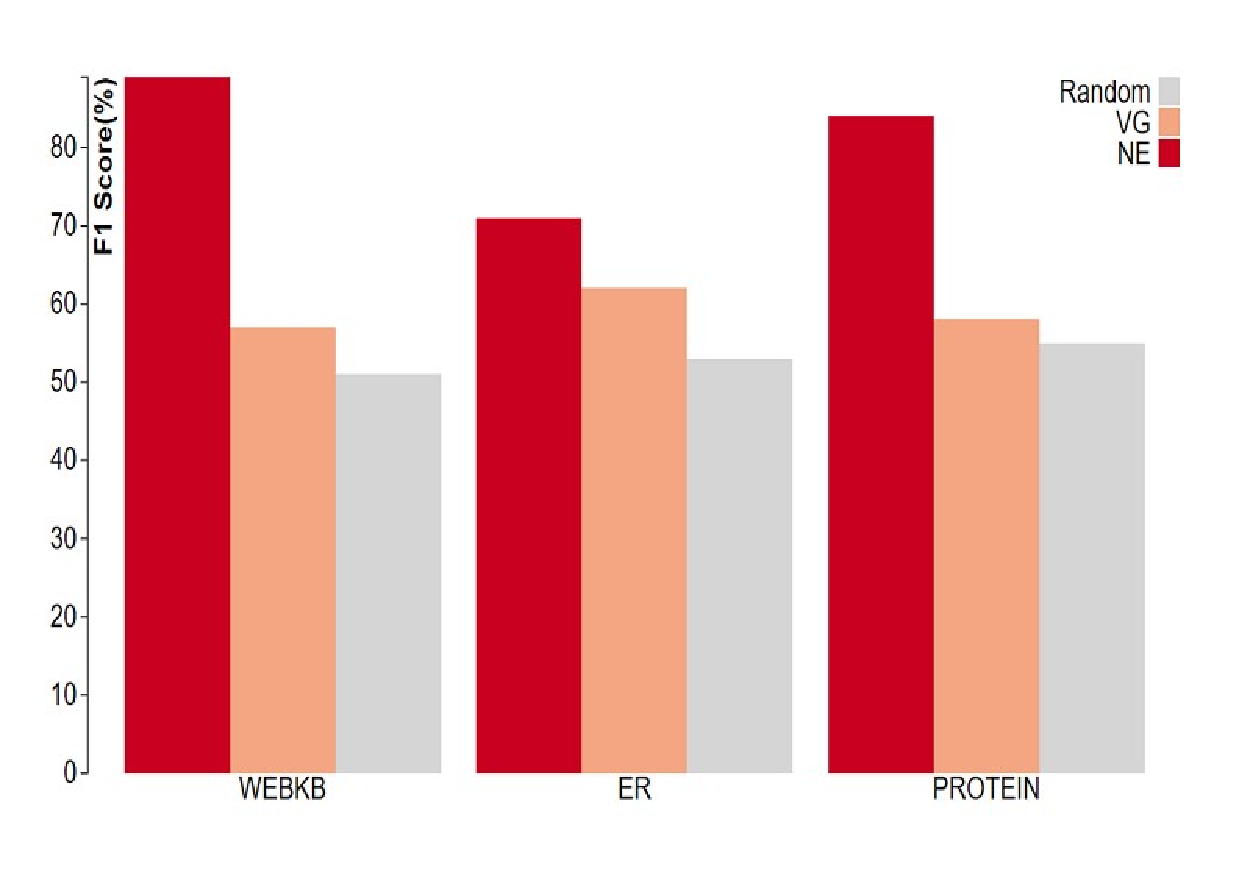
\includegraphics[scale=0.40]{quality.pdf}
\caption{\small{\label{fig:quality} Comparison of F-measures of approximate results on benchmarks using various approaches, as compared to the gold standard  (GS) results.}}
\end{figure}

\subsubsection{Symmetry Detection}

We evaluated the effect of increasing the context on symmetry detection. Specifically, we considered a simple synthetic MLN, where we incrementally add formulas of the form ${\tt R}(x)$ $\wedge$ ${\tt P}_i(x,y)$. Initially, we have a single formula, and add  evidences such that there is a common context for specific objects in $\Delta_x$. Our aim is to detect all those objects of $\Delta_x$ as being symmetric to each other. As we add more formulas, the common context for the symmetric objects in $\Delta_x$ keeps increasing. Fig.~\ref{fig:symmetry} shows our results in terms of the $\%$ of symmetric objects we could detect as we increase the number of formulas, i.e., as we add ${\tt R}(x)$ $\wedge$ ${\tt P}_1(x,y)$, ${\tt R}(x)$ $\wedge$ ${\tt P}_2(x,y)$, etc. Our results clearly shows that as the amount of context for symmetric objects in $\Delta_x$ increases, symmetry detection becomes more accurate.

%To do this, for every object, we obtained the list of similar objects in the embedding, and considered these as symmetric objects
\begin{figure}
  \centering
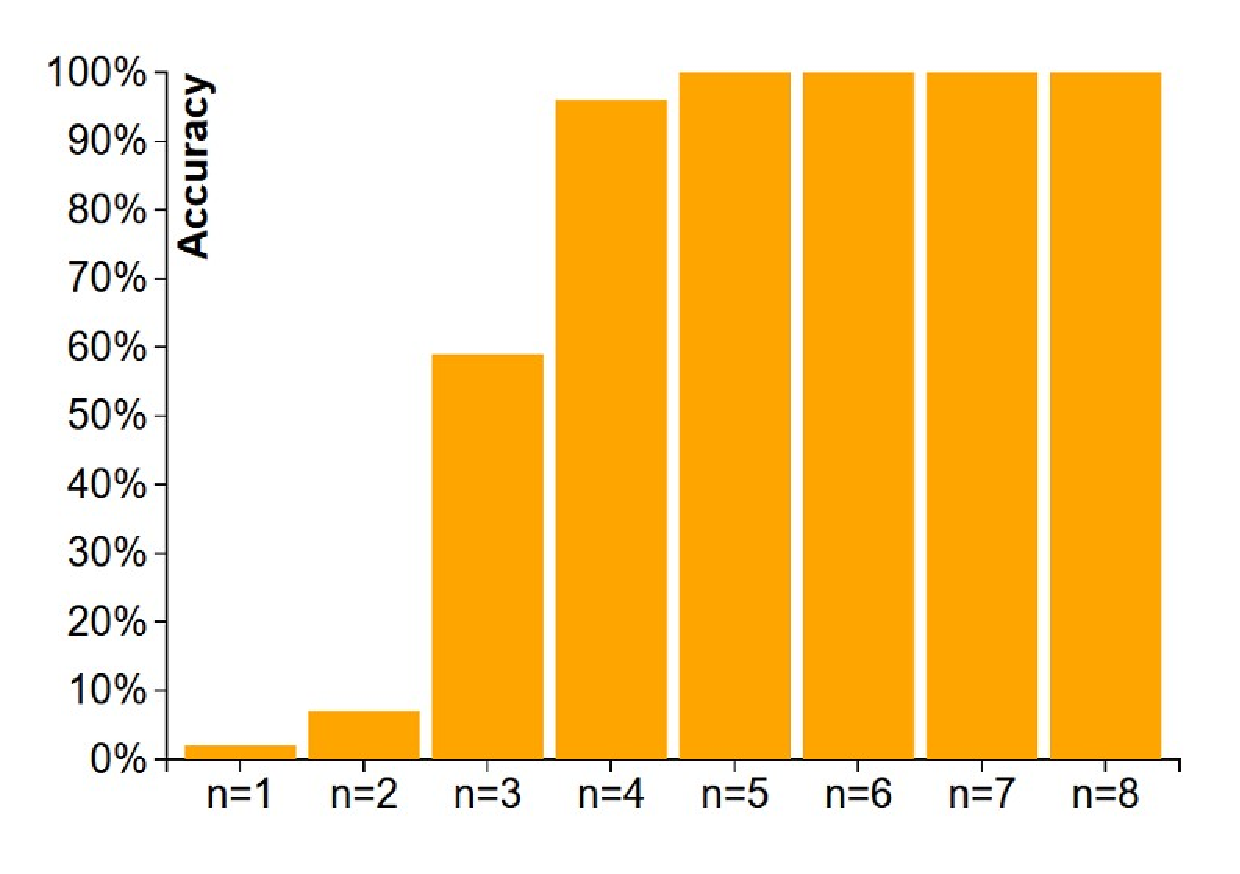
\includegraphics[scale=0.40]{symmetry.pdf}
\caption{\small{\label{fig:symmetry} Accuracy in detecting symmetries as we increase the context.}}
\end{figure} 

Next, we considered the effect of joint dependencies among multiple domains. Specifically, we analyzed the correlation between the symmetry of one domain and the symmetry of other, related domains. For this, we used a real-world dataset consisting of reviews from Yelp. Specifically, we used 7000 reviews written by around 200 users regarding around 800 restaurants.  Each review had a score (between 1 and 5) given by a user, and each review was written for a specific restaurant. For our experiment, we considered a simple MLN structure: ${\tt Word}$ ($review$,$word$) $\wedge$ ${\tt User}$ ($review$, $user$) $\wedge$ ${\tt Rest}$ ($review$, $restaurant$) $\Rightarrow$ ${\tt Score}$ ($review$, $score$). We embed the domain objects using Obj2vec, and then for each review $R$, we computed $k$ of its closest neighbors in the embedding. For each of $R$'s neighbors, we computed the similarity between the review vectors, the similarity between user vectors corresponding to users who wrote the reviews, and the similarity between restaurant vectors corresponding to restaurants about which the reviews were written. We then averaged these similarity values over all reviews over varying values of $k$ (between 1 to 10). As shown by the results in Fig~\ref{tab:score}, symmetries in the reviews, closely correlates to symmetries on the user who wrote the reviews, and symmetries on the restaurants for which the review was written. As our neighborhood size increases, the similarity scores go down uniformly. Thus, each variable's symmetry has a dependency upon the other variables.

%Then we applied our NE on this MLN with the purpose that symmetric reviews should have similar restaurants and users as NE considers joint dependency among domains.


\eat{
To ascertain our claim, we created an arbitrary MLN having $f_1$ $\ldots$ $f_n$ formulas of the form ${\tt R}(x)$ $\wedge$ ${\tt S}(x,y)$. Then we added symmetric evidence atoms like ${\tt R}(x_i)$,${\tt S}(x_i,y_j)$ where ${\tt i}$ $\%$ ${\tt k}$  = ${\tt j}$ for any constant ${\tt k}$. We added symmetric atom this way to test whether our NE can identify the symmetry. We noticed that NE accuracy increases as we increase number of formulas. Fig.~\ref{fig:symmetry} shows that accuracy becomes 100$\%$ for ${\tt n}$=5.
}



 



\eat{
\begin{table}[]
  \centering
  \fontsize{20}{9}\selectfont
  \resizebox{0.47\textwidth}{!}{
 %\tabcolsep=0.15cm
\begin{tabular}{| c | c | c | c |}
\hline
\rule{0pt}{20pt}\textbf{Review} & \textbf{Review Score} & \textbf{User Score} & \textbf{Rest Score}\\[0ex]
\hline
\rule{0pt}{20pt}Review 1   &   0.73 & 0.86 & 0.99 \\[0ex]
\rule{0pt}{20pt}Review 3   &   0.72 & 0.96 & 0.99 \\[0ex]
\rule{0pt}{20pt}Review 3   &   0.70 & 0.98 & 0.99 \\[0ex]
\rule{0pt}{20pt}Review 4   &   0.67 & 0.91 & 0.99 \\[0ex]
\rule{0pt}{20pt}Review 5   &   0.66 & 0.88 & 0.98 \\[0ex]
\rule{0pt}{20pt}Review 6   &   0.66 & 0.98 & 0.99 \\[0ex]
\rule{0pt}{20pt}Review 7   &   0.63 & 0.98 & 0.99 \\[0ex]
\rule{0pt}{20pt}Review 8   &   0.60 & 0.97 & 0.99 \\[0ex]
\rule{0pt}{20pt}Review 9   &   0.60 & 0.76 & 0.99 \\[0ex]
\rule{0pt}{20pt}Review 10   &   0.60 & 0.94 & 0.99 \\[0ex]
\hline
\end{tabular}
  }
  \normalsize
  \caption {\label{tab:score}Comparison of similarity scores of top 10 reviews and their respective users and restaurants.}
\end{table}
}

\begin{table}[]
  \centering
  \fontsize{20}{9}\selectfont
  \resizebox{0.47\textwidth}{!}{
 %\tabcolsep=0.15cm
\begin{tabular}{| c | c | c | c |}
\hline
\rule{0pt}{20pt}\textbf{ Nearest reviews ($k$)} & \textbf{Avg Review Sim} & \textbf{Avg User Sim} & \textbf{Avg Rest Sim}\\[0ex]
\hline
\rule{0pt}{20pt} 1   &   1.00 & 0.99 & 1.00 \\[0ex]
\rule{0pt}{20pt} 2   &   0.73 & 0.99 & 0.99 \\[0ex]
\rule{0pt}{20pt} 3   &   0.70 & 0.91 & 0.89 \\[0ex]
\rule{0pt}{20pt} 4   &   0.60 & 0.71 & 0.78 \\[0ex]
\rule{0pt}{20pt} 5   &   0.59 & 0.71 & 0.78 \\[0ex]
\rule{0pt}{20pt} 6   &   0.58 & 0.72 & 0.78 \\[0ex]
\rule{0pt}{20pt} 7   &   0.57 & 0.68 & 0.71 \\[0ex]
\rule{0pt}{20pt} 8   &   0.55 & 0.72 & 0.68 \\[0ex]
\rule{0pt}{20pt} 9   &   0.51 & 0.7 & 0.72 \\[0ex]
\rule{0pt}{20pt} 10  &   0.50 & 0.67 & 0.71 \\[0ex]
\hline
\end{tabular}
  }
  \normalsize
  \caption {\label{tab:score}Average similarity score of reviews, users and restaurants as we increase number of nearest reviews.}
\end{table}

\subsubsection{Scalability}

\eat{
Fig.~\ref{fig:time} illustrates required time for compression and inference as our ultimate goal is to reduce time. Fig.~\ref{fig:time}, exhibits that our NE takes almost similar time compared to VG and Random while compression time for each approach is trivial but inference takes notably less time compared to GS which makes our approach scalable and practical.
 }
 We evaluate scalability of our approach in terms of time required to generate the embedding and reduce the objects, as well as time for inference on the reduced MLN. Fig.~\ref{fig:time} shows our results for time required to generate the reduced MLN. Here, NE takes slightly longer than VG for reducing the MLN on the WebKB and ER datasets, and is almost the same for the protein dataset. The inference time on the reduced MLN was nearly the same for both NE and VG.
\begin{figure}
  \centering
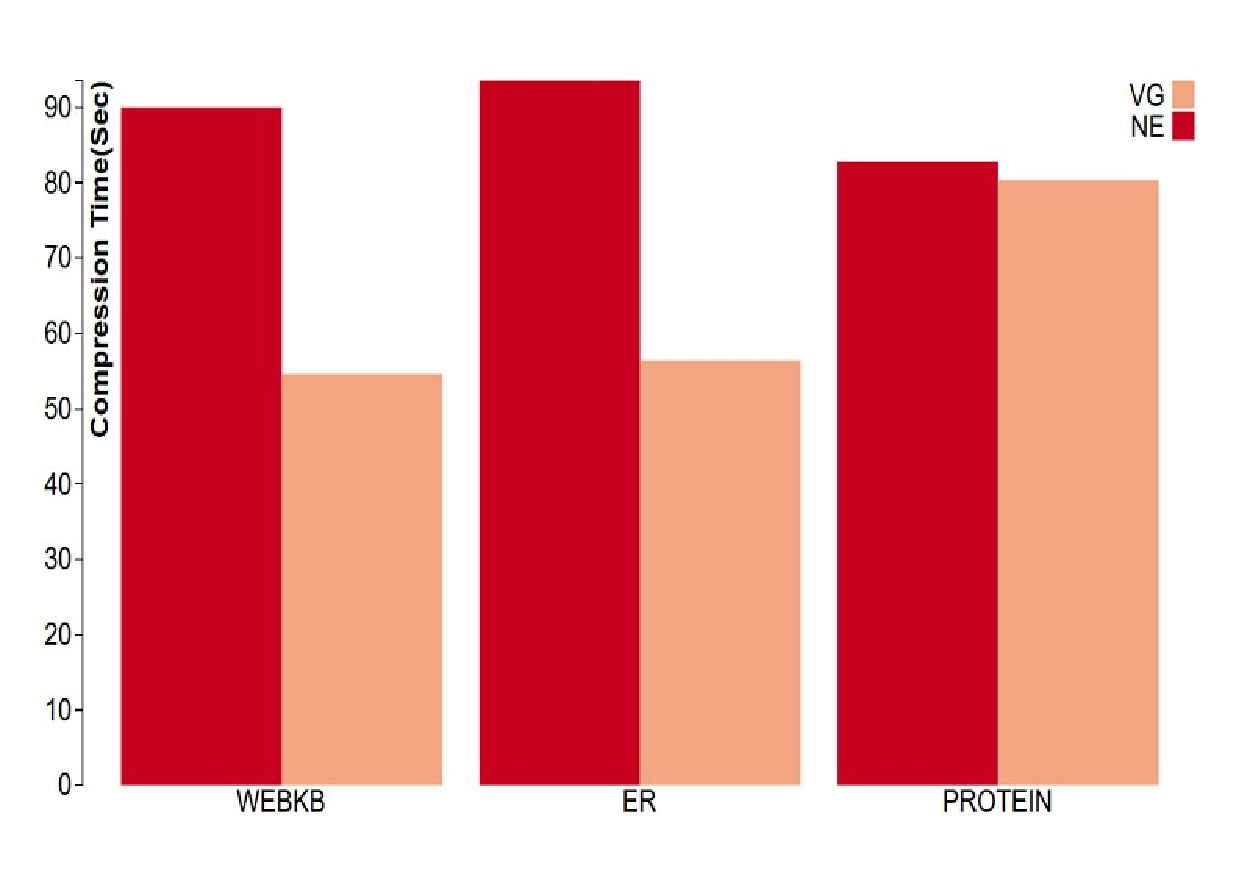
\includegraphics[scale=0.40]{compress_time.pdf}
\caption{\small{\label{fig:time} Comparison of running time for NE and VG.}}
\end{figure}

\eat{
\begin{figure}
  \centering
\includegraphics[scale=0.40]{inference.pdf}
\caption{\small{\label{fig:time} Comparison of compression and inference time for GS, NE, VG and Random.}}
\end{figure}
}
\section{Conclusion}

In this paper, we presented a novel approach to perform approximate lifted inference in MLNs by leveraging neural embeddings. Specifically, our idea was to exploit the fact that objects with similar contexts (other objects that appear with the object in ground formulas), are likely to be symmetric. Therefore, we encoded the context of an object and trained a neural network on this encoding such that the hidden layer embeds objects in a low-dimensional vector space, where similar objects lie close to each other in this space. We then reduced the number of objects in the MLN by retaining a subset of objects that are close in the embedded-space to the remaining objects that were eliminated from the MLN. Our experiments on real-world datasets showed that our approach is efficient and accurate.

Future work includes leveraging neural models to perform weight and structure learning in MLNs.
%% The file named.bst is a bibliography style file for BibTeX 0.99c
%\bibliographystyle{named}
 \bibliographystyle{plain}
\bibliography{all}

\end{document}

